\documentclass[tikz,border=5pt]{standalone}
\usepackage[UTF8]{ctex}
\usepackage{amsmath,amssymb}
\usetikzlibrary{arrows.meta,calc}
\tikzset{>=Stealth,line cap=round,line join=round,
motion/.style={blue!75!black,thick},
relative/.style={orange!85!black,thick},
electric/.style={red!70!black,thick},
aux/.style={gray!65,dashed,thin}}
\newcommand{\electron}[1]{\filldraw[fill=white,thick]#1 circle(.075);}
\begin{document}
% 1. The left/right electrons are explicitly numbered. B points out of the plane.
\begin{tikzpicture}[font=\small]
\begin{scope}
\draw[aux](-1.6,0)--(1.6,0);
\electron{(-1.6,0)} \electron{(1.6,0)}
\node[below left]at(-1.6,-.08){$2$};
\node[below right]at(1.6,-.08){$1$};
\draw[motion,->](1.6,.1)--(1.6,1.15)node[above]{$v_0$};
\draw[motion,->](-1.6,-.1)--(-1.6,-1.15)node[below]{$v_0$};
\draw[<->](-1.6,-1.67)--(1.6,-1.67)node[midway,below]{$l$};
\node at(0,1.20){$\odot\ B_0$};
\node at(0,1.90){（1）等大反向};
\end{scope}
\begin{scope}[xshift=5.9cm]
\draw[aux](-1.6,0)--(1.6,0);
\electron{(-1.6,0)} \electron{(1.6,0)}
\node[below left]at(-1.6,-.08){$2$};
\node[below right]at(1.6,-.08){$1$};
\draw[motion,->](1.6,.1)--(1.6,1.15)node[above]{$v_0$};
\node[left]at(-1.78,.35){$\boldsymbol v_2=0$};
\draw[<->](-1.6,-1.67)--(1.6,-1.67)node[midway,below]{$l$};
\node at(0,1.20){$\odot\ B_0$};
\node at(0,1.90){（2）仅电子 $1$ 初始运动};
\end{scope}
\draw[->](3,-1.20)--(3.75,-1.20)node[right]{$x$};
\draw[->](3,-1.20)--(3,-.48)node[above]{$y$};
\end{tikzpicture}
% 2. Actual forces: magnetic force in, electric repulsion out.
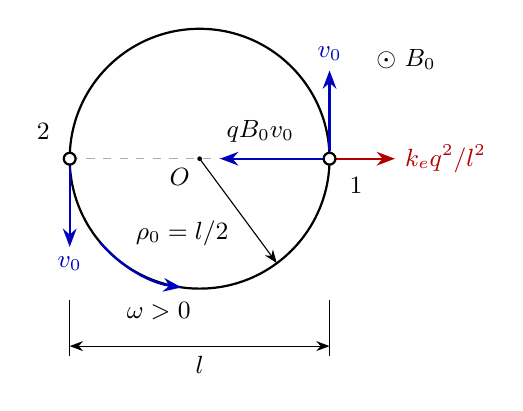
\begin{tikzpicture}[font=\small]
\draw[thick](0,0)circle(1.65);
\draw[aux](-1.65,0)--(1.65,0);
\fill(0,0)circle(.03)node[below left]{$O$};
\draw[thin,->](0,0)--(.98,-1.326)node[midway,below left]{$\rho_0=l/2$};
\draw[motion,->](1.65,.1)--(1.65,1.12)node[above]{$v_0$};
\draw[motion,->](-1.65,-.1)--(-1.65,-1.12)node[below]{$v_0$};
\draw[motion,->](1.65,0)--(.26,0);
\node[above]at(.77,.08){$qB_0v_0$};
\draw[electric,->](1.65,0)--(2.48,0)node[right]{$k_eq^2/l^2$};
\electron{(1.65,0)} \electron{(-1.65,0)}
\node[below right]at(1.78,-.12){$1$};
\node[above left]at(-1.78,.12){$2$};
\draw[motion,->](-1.264,-1.061)arc(220:262:1.65);
\node at(-.52,-1.93){$\omega>0$};
\draw[thin](-1.65,-1.80)--(-1.65,-2.50);
\draw[thin](1.65,-1.80)--(1.65,-2.50);
\draw[<->](-1.65,-2.38)--(1.65,-2.38)node[midway,below]{$l$};
\node at(2.62,1.26){$\odot\ B_0$};
\end{tikzpicture}
% 3. Symmetric radial perturbation. Only genuine forces have force arrows.
\begin{tikzpicture}[font=\small]
\begin{scope}
\draw[aux](0,0)circle(1.25);
\draw[thick](0,0)circle(1.65);
\draw[thin](0,0)--(1.65,0);
\fill(0,0)circle(.03)node[below left]{$O$};
\draw[fill=gray!15](1.25,0)circle(.045);
\node[above]at(.64,.1){$\rho_0$};
\electron{(-1.65,0)} \electron{(1.65,0)}
\node[below left]at(-1.78,-.10){$2$};
\node[below right]at(1.78,-.10){$1$};
\draw[motion,->](1.65,.10)--(1.65,1.04)node[above]{$v(x)$};
\draw[thin](0,-1.86)--(0,-2.27);
\draw[thin](1.65,-1.86)--(1.65,-2.27);
\draw[<->](0,-2.15)--(1.65,-2.15)node[midway,below]{$\rho=\rho_0(1+x)$};
\node at(0,2.05){虚线：未扰动圆；实线：$\rho>\rho_0$};
\end{scope}
\begin{scope}[xshift=5.9cm]
\draw[->](-.5,1.18)--(.65,1.18)node[right]{$+\rho$};
\draw[motion,->](0,0)--(-1.52,0)node[left]{$m\Omega v$};
\draw[electric,->](0,0)--(1.02,0)node[right]{$k_eq^2/(4\rho^2)$};
\electron{(0,0)}
\draw[motion,->](0,.12)--(0,.83)node[right]{$v$};
\node at(0,-.72){$m\ddot\rho=mv^2/\rho+F_{\rm e}-F_{\rm B}$};
\node[align=center]at(0,-1.45){$mv^2/\rho$ 来自加速度移项\\不是额外相互作用};
\node at(0,2.05){电子 $1$ 的径向方程};
\end{scope}
\end{tikzpicture}
% 4. Exact sample geometry: omega/Omega=.4, Omega*t=50deg.
% l=4cm, rho=2cm, a_c=.8cm; centers and endpoints follow the actual equations.
\begin{tikzpicture}[font=\small,scale=1.2]
\coordinate(G)at(-.8,0);
\coordinate(O)at(0,0);
\coordinate(C)at({.8*(cos(50)-1)},{.8*sin(50)});
\coordinate(P1)at({.8*(cos(50)-1)+2*cos(20)},{.8*sin(50)+2*sin(20)});
\coordinate(P2)at({.8*(cos(50)-1)-2*cos(20)},{.8*sin(50)-2*sin(20)});
\draw[motion](G)circle(.8);
\draw[aux](C)circle(2);
\draw[relative,thin](P2)--(P1);
\draw[relative,->](C)--(P1)node[midway,above]{$l/2$};
\draw[motion,thin](G)--(C);
\node[motion,below right]at($ (G)!.46!(C) $){$a_c$};
\draw[thin](G)--(O);
\draw[motion,->]({-.8+.8*cos(90)},{.8*sin(90)})
arc[start angle=90,end angle=145,radius=.8];
\node[motion]at(-1.64,1.02){$\Omega$};
\begin{scope}[shift={(C)}]
\draw[relative,->](130:2)arc[start angle=130,end angle=155,radius=2];
\node[relative]at(148:2.30){$\omega$};
\end{scope}
\fill(G)circle(.035)node[below left]{$G$};
\fill(O)circle(.035)node[below right]{$O$};
\fill(C)circle(.04);
\node[above right]at({.8*(cos(50)-1)+.10},{.8*sin(50)+.18}){$M$};
\electron{(P1)} \electron{(P2)}
\node[above right]at(P1){$1$};
\node[below left]at(P2){$2$};
\node[motion]at(-.8,-.93){质心圆};
\node[align=center]at(.3,-1.83){$a_c=v_0/(2\Omega)$；橙色连线长度为 $l$};
\node at(.2,3.08){质心绕 $G$ 转，电子绕当前质心转};
\end{tikzpicture}
% 5. Velocity-space translations separate parallel vectors without false overlap.
\begin{tikzpicture}[font=\small]
\begin{scope}
\draw[motion,->](-.82,0)--(-.82,1.2)node[above]{$\boldsymbol V_c$};
\draw[relative,->](.82,0)--(.82,1.2)node[above]{$\boldsymbol u_1$};
\node at(-.82,-.29){$v_0/2$};
\node at(.82,-.29){$v_0/2$};
\draw[->,thick](2.06,0)--(2.06,2.4)node[above]{$\boldsymbol v_1$};
\node[right]at(2.12,1.12){$v_0$};
\node at(.6,-1.01){$t=0$，相位差为 $0$};
\node at(.6,3.12){两速度分量同向};
\end{scope}
\begin{scope}[xshift=6.7cm,yshift=.65cm]
\draw[motion,->](0,0)--(-1.47,-.49)node[below left]{$\boldsymbol V_c$};
\draw[relative,->](0,0)--(1.47,.49)node[above right]{$\boldsymbol u_1$};
\fill(0,0)circle(.035);
\node[motion,above]at(-.83,-.21){$v_0/2$};
\node[relative,below]at(.83,.21){$v_0/2$};
\node at(0,-1.0){$\boldsymbol v_1=\boldsymbol V_c+\boldsymbol u_1=0$};
\node at(0,-1.66){$(\Omega-\omega)t_*=\pi$};
\node at(0,2.47){首次相消；两分量等模反向};
\end{scope}
\end{tikzpicture}
\end{document}
